\documentclass[a4paper]{article}

%%%%%%%% BIBLIOGRAPHIE %%%%%%%%
%\usepackage[backend=biber]{biblatex} %Imports biblatex package  //version biber et pas biblatex, ne marche pas direct sur texmaker.
%\addbibresource{biblio.bib} %Import the bibliography file

%%%%%%% PACKAGE %%%%%%%%%%%

\usepackage[utf8]{inputenc}
\usepackage{xcolor}
\usepackage{amsmath}
\usepackage{amssymb}
\usepackage{amsfonts}
\usepackage{verbatim}
\usepackage{amsthm}
\usepackage{geometry}
\geometry{hmargin=2cm,vmargin=1.5cm}
\usepackage{hyperref}

%%%%% Pour les dessins %%%%%

\usepackage{tikz}
\usetikzlibrary{shapes,positioning}
\usetikzlibrary{calc}
\usetikzlibrary{matrix,arrows,patterns.meta}
\usepackage{graphicx}

\tikzset{
	c/.style={every coordinate/.try}
}

%%%%%%% THEOREM %%%%%%%%%%%%%%%%

\newtheorem{prop1}{Proposition}
\newtheorem{coro1}{Corollary}
\newtheorem{thm}{Theorem}
\newtheorem{def1}{Definition}
\newtheorem{lem1}{Lemma}
\newtheorem{rq1}{Remark}

%%%%%%%% NEW COMMANDS %%%%%%%%%


\newcommand{\calP}{\mathcal{P}}
\newcommand{\calH}{\mathcal{H}}
\newcommand{\calL}{\mathcal{L}}
\newcommand{\calC}{\mathcal{C}}
\newcommand{\calD}{\mathcal{D}}
\newcommand{\Tr}{\operatorname{Tr}}
\newcommand{\fqm}{\mathbb{F}_{q^m}}
\newcommand{\fq}{\mathbb{F}_{q}}
\newcommand{\Z}{\mathbb{Z}}
\newcommand{\R}{\mathbb{R}}

%%----Commentaires----%%%

\newcommand\jade[1]{\textcolor{purple}{#1}}
\newcommand\TODO[1]{\textcolor{red}{TO DO: #1}}


\title{Hermitian-SSAG-code distinguisher}
\author{Mathieu Lhotel}
\date{}

\begin{document}

\maketitle

\section{\textcolor{blue}{Introduction}}

\TODO{Définition de $\star$, code dual, Trace, SS...}



\textcolor{blue}{
	\begin{lem1} \label{known_bounds}
		Let $\calC$ and $\calD$ be two linear codes over $\fqm$ with same length $n$ and respective dimension $k_{\calC}$ and $k_{\calD}$. We have
		\begin{itemize}
			\item[$(1)$] $\dim_{\mathbb{F}_q}(\Tr(\calC)) \leq \min\{mk_{\calC},n\}$;
			\item[$(2)$] $\dim_{\fqm}(\calC \star \calD) \leq \min\{k_{\calC}k_{\calD},n\}$;
			\item[$(3)$] If $\calC$ is suffisciently random, we have
			\[ \dim_{\mathbb{F}_{q^m}}(\calC^{\star2}) \leq \mathrm{min}\left(n,\binom{k_{\calC}+1}{2}\right) . \]
			Espescially, if $\calC^{\star2}$ does not fill the full space, we expect to have 
			\[ \dim_{\mathbb{F}_{q^m}}(\calC^{\star2}) = \binom{k_{\calC}+1}{2}.\]
		\end{itemize}
	\end{lem1}
}
\textcolor{blue}{	
	\begin{prop1} [\cite{rocco} Corollary 16]\label{1st bound square of trace}
		Let $\calC$ be any $\fqm$-linear code. Then 
		\begin{equation} \label{bbbound}
			\dim_{\fq}(\Tr(\mathcal{C})^{\star2}) \leq m \cdot \dim_{\fqm}(\calC^{\star 2}) + \binom{m}{2} (\dim_{\fqm}(\calC))^2.
		\end{equation}
		Furthermore, if $\dim_{\fq} \Tr(\calC) = m \cdot \dim_{\fqm}(\calC)$, then 
		\[\dim_{\fq} (\Tr(\calC)^{\star 2}) - \binom{\dim_{\fq} \Tr(\calC)+1}{2} \leq m \cdot \dim_{\fqm} \calC^{\star 2} - \binom{\dim_{\fqm} (\calC)+1}{2}.\]
	\end{prop1}
}

\textcolor{blue}{\begin{thm} \label{th1}
		\jade{Ce sera défini avant : With usual definitions of the trace and the $\star$-product of codes,} we have 
		\[ \Tr(C)^{\star2} := ((C^{\perp}))^{\star2} \subseteq \sum\limits_{i=0}^{\lfloor{m/2} \rfloor} \Tr(C\star C^{q^i}),\]
		where $C^{\perp}$ is the dual code of $C$. \\
		Moreover, if $m$ is even (which is the case in our settings), we have 
		\[\dim_{\mathbb{F}_q}(\Tr(C \star C^{q^{m/2}})) \leq \frac{m}{2}\cdot (\dim_{\fqm}(C))^2.\]
	\end{thm}
}

%\section{\textcolor{blue}{Preliminaries}}
\section{\textcolor{blue}{SSAG codes Distinguisher}}
\textcolor{blue}{AG codes}
\subsection{\textcolor{blue}{Hermitian codes and their subfield subcodes}}

The goal of this note is an adaptation of a distinguisher for alternant and Goppa codes (see \cite{rocco}) in the case of SSAG-Hermitian one-point code, whose divisor is either a multiple of $P_{\infty}$ or a multiple of a degree 3 place. \\
We work on the finite field $\mathbb{F}_{q^m}=\mathbb{F}_{q_0^2}$, were $q$ is a prime power. We denote by $\calH = \mathbb{F}_{q_0^2}(x,y)$ the Hermitian function field, defined by 
\[ y^{q_0}+y=x^{q_0+1}.\]

\textcolor{blue}{The goal of this work is to adapt the distinguisher given in \cite{rocco} of alternant and Goppa codes for the subfield subcodes of $1-$point Hermitian code, whose divisor is a multiple of $P_{\infty}$. (Hermitian code definition should be given in the previous subsection) To ensure consistency in our notation, we do the following conventions. Let $\mathbb{F}_{q^m}=\mathbb{F}_{q_0^2}$, were $q$ is a prime power. We denote by $\calH = \mathbb{F}_{q_0^2}(x,y)$ the Hermitian function field, defined by 
	\[ y^{q_0}+y=x^{q_0+1}.\] }

\textcolor{blue}{(Throughout this paper) Let $\mathcal{C} := C_{\calL}(\calH,\mathcal{P},D)$ be an AG-code defined over $\calH$, where $D=sP_{\infty}$. To establish a disinguisher, we set the following result, which is a consequence of Delsarte's Theorem and Rocco's estimate (see \cite{rocco}, Proposition 15)}.


Throughout this paper, let
\[\mathcal{C} := C_{\calL}(\calH,\mathcal{P},D) \]
be an AG-code defined over $\calH$, where $D=sP_{\infty}$ or $D=sP$; $P$ being any degree 3 place on $\calH$. 
In order to get a disinguisher, we start from the following result, which is a consequence of Delsarte's Theorem and Rocco's estimate (see \cite{rocco}, Proposition 15)

\textcolor{blue}{
	\begin{thm} \label{th1}
		With usual definitions of the trace and the $\star$-product of codes, we have 
		\[ \Tr(\mathcal{C})^{\star2} := (\mathrm{SSAG}_{q}(\calH,\calP,D')^{\perp})^{\star2} \subseteq \sum\limits_{i=0}^{\lfloor{m/2} \rfloor} \Tr(\mathcal{C}\star\mathcal{C}^{q^i}),\]
		where $D'$ is the dual divisor of D, which can be explicitly described using $\calP$ and $D$ (see \cite{sti}, Proposition 2.2.10). \\
		\jade{Pourquoi cette répétition ? $\rightarrow$}Moreover, if $m$ is even (which is the case in our settings), we have 
		\[\dim_{\mathbb{F}_q}(\Tr(\calC \star \calC^{q^{m/2}})) \leq \frac{m}{2}\cdot (\dim_{\fqm}(\calC))^2.\]
	\end{thm}
}


\begin{thm} \label{th1}
With usual definitions of the trace and the $\star$-product of codes, we have 
\[ \Tr(\mathcal{C})^{\star2} := (\mathrm{SSAG}_{q}(\calH,\calP,D^{\perp})^{\perp})^{\star2} \subseteq \sum\limits_{i=0}^{\lfloor{m/2} \rfloor} \Tr(\mathcal{C}\star\mathcal{C}^{q^i}),\]
where $D^{\perp}$ is the dual divisor of D, which can be explicitly described using $\calP$ and $D$ (see \cite{sti}, Proposition 2.2.10). \\
Moreover, if $m$ is even (which is the case in our settings), we have 
\[\dim_{\mathbb{F}_q}(\Tr(\calC \star \calC^{q^{m/2}})) \leq \frac{m}{2}\cdot (\dim_{\fqm}(\calC))^2.\]
\end{thm}

\jade{ça doit dégager $\downarrow$}
{\color{red}

Before specifying to AG-codes, we also recall the following estimations (which can also be found in \cite{rocco}):

\begin{lem1} \label{known_bounds}
Let $\calC$ and $\calD$ be two linear codes over $\fqm$ with same length $n$ and respective dimension $k_{\calC}$ and $k_{\calD}$. We have
\begin{itemize}
    \item[$(1)$] $\dim_{\mathbb{F}_q}(\Tr(\calC)) \leq \min\{mk_{\calC},n\}$;
    \item[$(2)$] $\dim_{\fqm}(\calC \star \calD) \leq \min\{k_{\calC}k_{\calD},n\}$;
    \item[$(3)$] If $\calC$ is suffisciently random, we have
     \[ \dim_{\mathbb{F}_{q^m}}(\calC^{\star2}) \leq \mathrm{min}\left(n,\binom{k_{\calC}+1}{2}\right) . \]
     Espescially, if $\calC^{\star2}$ does not fill the full space, we expect to have 
     \[ \dim_{\mathbb{F}_{q^m}}(\calC^{\star2}) = \binom{k_{\calC}+1}{2}.\]
\end{itemize}
\end{lem1}
}

\jade{Blablabla: On veut voir si le dual reiste au square distinguisher donc on est amené à regarder des carrés de codes AG....}

It is well-known that (3) above does not hold if $\calC$ has too much structure, which is the case for Reed-Solomon codes and more generally for AG-codes.

\begin{prop1}[\cite{mumford}, Theorem 6] \label{prop1}
Let $F,G$ be two divisors in $\calH$ such that $\deg(G) \geq 2g(\calH)+1$ and $\deg(F) \geq 2g(\calH)$, where $g(\calH)$ is the genus of $\calH$. Then
\[ \calL(F) \cdot \calL(G) = \calL(F+G),\]
where $\calL(F) \cdot \calL(G) := \mathrm{span}_{\mathbb{F}_{q^m}}\{ f \cdot g : f,g \in \calL(F) \times \calL(G) \}$.\\ 
As a consequence, if $deg(D) \geq 2g(\calH)+1$, then 
\[ (C_{\calL}(\calH,\mathcal{P},D))^{\star2} = C_{\calL}(\calH,\calP,2D).\]
The Riemann-Roch theorem thus gives
\[ \dim_{\mathbb{F}_{q^m}}(C_{\calL}(\calH,\mathcal{P},D)^{\star2}) = 2\deg(D)+1-g(\calH)) = \deg(D) + \dim_{\fqm}(C_{\calL}(\calH,\mathcal{P},D)), \]
which is much smaller than the expected dimension given in Lemma \ref{known_bounds}, and thus provides a distinguisher for AG-codes.
\end{prop1}

In what follows, we will be interested in subfield subcodes of AG-code, meaning that we will rather need an estimation of the dimension of the square of a trace code (instead of the code itself). Theorem \ref{th1} can be used to get a first one, using the following Proposition from \cite{rocco}.

\begin{prop1} [\cite{rocco} Corollary 16]\label{1st bound square of trace}
Let $\calC$ be any $\fqm$-linear code. Then 
\begin{equation} \label{bbbound}
    \dim_{\fq}(\Tr(\mathcal{C})^{\star2}) \leq m \cdot \dim_{\fqm}(\calC^{\star 2}) + \binom{m}{2} (\dim_{\fqm}(\calC))^2.
\end{equation}
Furthermore, if $\dim_{\fq} \Tr(\calC) = m \cdot \dim_{\fqm}(\calC)$, then 
\[\dim_{\fq} (\Tr(\calC)^{\star 2}) - \binom{\dim_{\fq} \Tr(\calC)+1}{2} \leq m \cdot \dim_{\fqm} \calC^{\star 2} - \binom{\dim_{\fqm} (\calC)+1}{2}.\]
\end{prop1}

The above Proposition implies that if the dimension of a square code is smaller than we expect from a random code, namely
\[ \dim_{\fqm} (\calC^{\star 2}) < \binom{\dim_{\fqm} (\calC)+1}{2},\]
then this property survives for the trace code, \emph{\textit{i.e.}}
\[\dim_{\fq} (\Tr(\calC)^{\star 2}) < \binom{\dim_{\fq} \Tr(\calC)+1}{2}.\]

Proposition \ref{prop1} exactly says that under some condition on the degree of its divisor, the dimension of the square of an AG-code is smaller that expected. This is still the case for their trace codes, which are SSAG codes associated to the dual divisor.

\begin{coro1} \label{square_ssag_bound}
Let $\mathcal{C} := C_{\calL}(\calH,\mathcal{P},D)$ be a dimension $k$ AG-code on $\calH$ associated to a degree $s \geq 2g(\calH)+1$ divisor. We have 
\[ \dim_{\fq}(\Tr(\mathcal{C})^{\star2}) := \dim_{\fq} ((\mathrm{SSAG}_{q}(\calH,\calP,D^{\perp})^{\perp})^{\star2})  \leq \binom{mk+1}{2} - \dfrac{m}{2} (k(k-1)-2s).\]
\end{coro1}

\begin{proof}
From Proposition \label{Prop1}, we have $\dim_{\fqm}(\calC)^{\star2} = 2s+1-g = k+s$, since we have inequality in the Riemann-Roch theorem. Thus, \eqref{bbbound} from Proposition \ref{1st bound square of trace} leads to
\begin{align*}
    \dim_{\fq}(\Tr(\mathcal{C})^{\star2}) &\leq m(k+s) + \binom{m}{2}k^2 \\
                                        &= (2k+2s+mk^2-k^2) \dfrac{m}{2} \\
                                        &= (k(mk+1)-k^2+k+2s) \dfrac{m}{2} \\
                                        &= \binom{mk+1}{2} - \dfrac{m}{2}(k(k-1)-2s) .
\end{align*}
\end{proof}

In \cite{rocco}, the authors show that for a Goppa code $\calC = \mathbf{GRS}_r(x,y)$ defined over $\mathbb{F}_{q^m}$, where $y_i = 1/\Gamma(x_i)$ ($\Gamma$ being a degree $r$ polynomial), it holds
\[\Tr(\calC\star\calC) \subseteq \Tr(\calC\star\calC^{q}) \subseteq \cdots \subseteq \Tr(\calC\star\calC^{q^u}),\]
for any $0 \leq u \leq f$,
where $f :=\lfloor\log_q(r)\rfloor $, or even without the Trace operator in the case of RS-codes. This allow them to use more efficiently Thereom \ref{th1} to get a better bound. \\
Our plan is to show that the same kind of result still holds in the case of AG-codes over $\mathbb{F}_{q^m}$, and use it to improve the bound in Corollary \ref{square_ssag_bound}. In particular, some Magma experiments shows that for $\mathcal{C} := C_{\calL}(\calH,\mathcal{P},D)$ , some integer $f$, and $0 \leq i \leq f \leq \lfloor m/2 \rfloor$, we have
\begin{equation} \label{equality_of_codes}
 \calC \star \calC^{q^i} = \calC^{q^i+1},
\end{equation}
which is equivalent to the equality of Riemann-Roch spaces
\[ \calL(D) \cdot \calL(D)^{q^i} = \calL((q^i+1)D).\]
In fact, if \eqref{equality_of_codes} holds, thus since 
$\calC^{q^i+1} \subseteq \calC^{q^{i+1}+1}$ is true for every integer $i$, the sequence of inclusions 
\[\calC\star\calC \subseteq \calC\star\calC^{q} \subseteq \cdots \subseteq \calC\star\calC^{q^f}\]
also holds (with traces as well), and can be used to refine the estimation of the dimension of $\Tr(\calC)^{\star2}$ by rewriting Theorem \ref{th1} as follows:

\begin{equation}\label{eq:dim_tr_inclusion}
	\Tr(\mathcal{C})^{\star2}:=\Tr(\mathcal{C} \star \mathcal{C}^{q^f}) + \sum_{i= f+1}^{\frac{m}{2}} \Tr(\mathcal{C} \star \mathcal{C}^{q^i}).
\end{equation}
In what follows, we will study \eqref{equality_of_codes}, starting by noting: 

\begin{lem1} \label{lemma1}
For every integer $i \geq 0$, we have
\[\calL(D) \cdot \calL(D)^{q^i} \subseteq \calL((q^i+1)D)\]
\end{lem1}

It remains to show in which conditions (on the degree of $D$ and the integer $i$), the reverse inclusion is also true. To study this, we specify the divisor $D$ as a multiple of the point at infinity or a degree 3 place, as these divisors give the most usable SSAG-codes. Section 2 is dedicated to the classical one-point Hermitian code whereas section 3 deals with degree 3 places.


\section{The case $D=sP_{\infty}$}

In this section, we fix $D=sP_{\infty}$, where $s=\deg(D)$. Note that in this case of a one-point Hermitian codes, the dual divisor $D^{\perp}$ has been explicitly described in \cite{sabi}, Theorem 3.2. In particular, if we set $s' := q_0^3+q_0^2-q_0-2-s$, then $D^{\perp} = s'P_{\infty}$. This fact is really important since in the end, we want to deal with \textrm{SSAG}-codes, and the one of interest in Theorem \ref{th1} is 
\[\mathrm{SSAG}_{q}(\calH,\calP,D^{\perp}),\]
i.e. we will have a result on the dimension of the square of its dual. We will come back at it later, but for the moment we will focus on finding a conditions to have equality on the inclusion in Lemma \ref{lemma1}. 

\noindent It is well-knonw from the study of the Hermitian curve that
\begin{equation} \label{rr_p_inf}
\calL(sP_{\infty}) = \langle x^iy^j : 0 \leq j \leq q_0-1 \ \mathrm{and} \ iq_0+j(q_0+1) \leq s \rangle_{\mathbb{F}_{q_0^2}}
\end{equation}

Recall that we want to find conditions on the integers $s$ and $i$ in order to have 
\begin{equation} \label{equality}
\calL(sP_{\infty}) \cdot \calL(sP_{\infty})^{q^i} = \calL((q^i+1)sP_{\infty})  
\end{equation}

\begin{rq1}
Keep in mind the difference between $q$ and $q_0$. More precisly, $q_0$ is the degree of the Hermitian curve over the rational function field, which is in the definition of our Riemann-Roch spaces. On the other side, $q$ is the cardinality of the field where our subfield subcode is considered. We have $q^{\frac{m}{2}}=q_0$.
\end{rq1}

Since the inclusion "$\subseteq$" in \eqref{rr_p_inf} is true for any $i \geq 0$, it remains to find a sufficient condition to have the reverse inclusion. To do so, the idea is to work with valuation (at $P_{\infty}$) of functions in both sides. Before going further into details, let us recall some fact about Weierstrass gap theory in this context (see \cite{sti} for more details).
Let $\calH(P_{\infty})$ be the Weierstrass semi-group at $P_{\infty}$, given by
\[\calH(P_{\infty}) = \langle q_0,q_0+1 \rangle_{\mathbb{N}};\]
and denote by  $\mathcal{G}(P_{\infty})$ the set of gap numbers such that
\[\calH(P_{\infty}) = \mathbb{N} \backslash \mathcal{G}(P_{\infty})\]
and 
\[\mathcal{G}(P_{\infty}) = \{1,...,q_0-1,q_0+2,...,2q_0-1,...,2g-1=q_0(q_0-1)-1\}.\]
It is well-known from this theory that $\mathcal{G}(P_{\infty})$ is a finite set of cardinality $g:=g(\calH) := \dfrac{q_0(q_0-1)}{2}$, the genus of $\calH$. For simplicity in the upcoming proofs, we will write 
\[\mathcal{G}(P_{\infty}) = \{\mu_1,\cdots,\mu_g\}.\]
Now we are ready to define the set of valuations we will work with: for any integer $i \geq 0$, define

\[A^s_{i,q}:=\{-\nu_{P_{\infty}}(h) : h \in \calL((q^i+1)sP_{\infty}) \}\] 
the set of all possible valuations at $P_{\infty}$ atteigned by any function in $\calL((q^i+1)sP_{\infty}$ (we put a "minus sign" to make it more readable, \emph{i.e.} we work with positive integers instead of negative ones, since $P_{\infty}$ is a pole of all functions we work with). Replacing $s$ by $(q^i+1)s$ in \eqref{rr_p_inf} yields
\[A^s_{i,q} = \calH(P_{\infty}) \cap \{1,\cdots,(q^i+1)s\} := \calH(P_{\infty})_{\leq s(q^i+1)}.\]
 We also introduce the set 
\[V^s = \{-\nu_{P_{\infty}}(f) : f \in \calL(sP_{\infty})\} := \calH(P_{\infty})_{\leq s},\]
the equality coming from $\eqref{rr_p_inf}$ as well. \\
A sufficient condition to have $\calL(sP_{\infty}) \cdot \calL(sP_{\infty})^{q^i} \supseteq \calL((q^i+1)sP_{\infty})$ is to prove that every integer in the set $A_i^s$ is attained as minus a valuation at $P_{\infty}$ of a function in the product space $\calL(sP_{\infty}) \cdot \calL(sP_{\infty})^{q^i}$, because this implies an equality of dimension between the two vector spaces (note that the corresponding dimension is the cardinality of the set $A_i^s$). Since 
\[\calL(sP_{\infty}) \cdot \calL(sP_{\infty})^{q^i} := \mathrm{span}_{\mathbb{F}_q^m}\{f \cdot g^{q^i} : (f,g) \in \calL(sP_{\infty})\}\]
exactly attains the valuations in the set $V^s+q^iV^s$,
we are led to find a condition such that 
\begin{equation} \label{equalitu_of_valuations}
    V^s+q^iV^s = A^s_{i,q}
\end{equation}
holds. Again, the natural inclusion on the corresponding Riemann-Roch spaces implies that  $V^s+q^iV^s \subseteq A^s_i$ is always true, \emph{i.e.} we only have to find a condtion to guaranty the reverse inclusion. \\
In fact, we start to proof a characterization of this in the case where we take powers of $q_0$ instead of $q$. It will be used later to get back to the case of interest.

\begin{prop1} \label{result_with_valuations}
Let $i > 0$. We have 
\[s \geq \mu_g + q_0^{i+1} \iff A^s_{i,q_0} := \calH(P_{\infty})_{\leq s(q_0^i+1)} = V^s+q_0^iV^s,\]
 where $\mu_g := 2g-1$ is the largest gap of $P_{\infty}$. In this case, we have 
 \[ \calC \star \calC^{q_0^i} = \calC^{q_0^i+1}.\]
\end{prop1}

\begin{proof} The case $i=0$ is given by Proposition \ref{prop1}, so let us suppose that $i \geq 1$. \\
We start by proving $(\Leftarrow)$, supposing by contraposition that $s < \mu_g + q_0^{i+1}$. In this case, we show that the element $\mu_g + q_0^{i+1} \in A^s_{i,q_0} \backslash V^s+q_0^iV^s$: it is clear that $\mu_g + q_0^{i+1} \notin V^s$ since it is striclty bigger than $s$, and that $\mu_g = q_0(q_0-1)-1$ yields
\[\mu_g + q_0^{i+1}=q_0^2-(q_0+1) + q_0^{i+1} < 2q_0^{i+1},\]
since $i \geq 1$. There is only two ways to decompose $\mu_g + q_0^{i+1}$ in $V^s+q_0^iV^s$ , the first one being the trivial one, \emph{i.e.}
\[\mu_g + q_0q_0^{i} \notin V^s+q_0^iV^s,\]
which doesn't work because $\mu_g \notin V^s$ since it is a gap. Remark that we can not decrease the $q_0^iV^s$ part without getting a gap, since $q_0 = \min{V^s}$. It means that we have to decrease it, by writting 
\[\mu_g + q_0^{i+1} = (\mu_g - q_0^i) + \underbrace{q_0^i(q_0+1)}_{\in q^i_0V^s} .\]
Here, we have $\mu_g - q_0^i = q_0^2-(q_0+1)-q_0^i <0 \notin V^s$, unless eventually $i=1$. But in the latter case, we easyly see that $\mu_g-q_0 = \mu_{g-1}$ is the $g-1$-th gap of $P_{\infty}$, and thus not in $V^s$. This proves that $\mu_g + q_0^{i+1} \notin V+q_0^iV$, and thus $(\Rightarrow)$. \\

In order to prove $(\Rightarrow)$, suppose $s \geq \mu_g+q_0^{i+1}$ and we show that $A^s_{i,q_0} \subseteq V^s+q_0^iV^s$. For that, let $a \in A^s_{i,q_0}$. There are a few cases to consider:
\begin{enumerate}
    \item if $a \leq s$, then by definition $a \in V^s$ (note that $a$ can not be a gap since it is in $A^s_{i,q_0}$). In this case we have  $a=a+0 \in V^s+q^i_0V^s$;
    \item else, $a > s \geq \mu_g+q_0^{i+1}$. In this case, there exist two integers $\alpha$ and $\beta$ such that 
     \[ a= \alpha q_0^{i+1} + \beta \ , \ 0 \leq \beta < q_0^{i+1}.\] 
     Now, there is a few cases to consider :
\begin{itemize}
    \item[(i)] \underline{$\beta > \mu_g$} : By definition, we have $a \leq s(q_0^i+1)$, meaning with the previous decomposition that $\alpha q_0 \leq s + \left\lfloor \frac{s-\beta}{q_0^i}\right\rfloor$. 
    \begin{itemize}
        \item[$\star$] If $\alpha q_0 \leq s$, then $a = (\alpha q_0)q_0^i + \beta$ is a valid decomposition of $a$ in $q_0^iV^s + V^s$, since $\mu_g < \beta < q_0^{i+1} < s$;
        \item[$\star$] Else, we have $\alpha q_0 > s$. In this case, write
        \begin{align*}
            a &= (\alpha q_0 - (\alpha q_0 - s))q_0^i + \underbrace{(\beta + (\alpha q_0 -s)q_0^i)}_{:=\beta'} = sq_0^i + \beta'.
        \end{align*}
        Since $\beta > \mu_g$ and $a \leq s(q_0^i+1)$, we conclude $\mu_g < \beta' \leq s$, and thus we have a valid decomposition for $a$ in this case.
    \end{itemize}
    \item[(ii)] \underline{$\beta \leq \mu_g$} : In this case, we start by writting
    \[ a = ((\alpha-1)q_0)q_0^i + (\beta+q_0^{i+1}) .\]
    Since $i\geq 1$, we know that $q_0^{i+1} \geq q_0^2 > \mu_g$, so we have $\mu_g < \beta+q_0^{i+1} \leq s$. At this point, there is still two cases to consider :
    \begin{itemize}
        \item [$\star$] $(\alpha-1)q_0 \leq s$; in which case the above decomposition of $a$ works;
        \item [$\star$] Else, $(\alpha-1)q_0 >s$. In this case, by setting $\beta'':= \beta + q_0^{i+1}+((\alpha-1)q_0-s)q_0^i$, we can write
        \[ a = ((\alpha-1)q_0 - ((\alpha-1)q_0-s)q_0^i + \beta'' = sq_0^i + \beta''.\]
        But clearly, $\beta'' > \beta + q_0^{i+1} > \mu_g$, and $a \leq s(q_0^i+1)$ implies $\beta'' \leq s$ also, which proves that the above decomposition works for $a$ in theses settings.
    \end{itemize}
From now on, the equality on codes follows immediatly.
\end{itemize}
    % In this case, there exist two integers $\alpha$ and $\beta$ such that 
    % \[ a= \alpha q_0^{i+1} + \beta \ , \ 0 \leq \beta < q_0^{i+1}.\]
    % To prove this decomposition is valid, it remains to prove that $\alpha q_0 \leq s$ and $\beta > \mu_g$ (since we already have $\beta \leq s$, and obviously $\alpha q_0 \in \calH(P_{\infty})$). 
    % \begin{itemize}
    %     \item [$\star$] By definition, $a \leq s(q_0^i+1)$, so we get
    %     \begin{align*}
    %         & (\alpha q_0)q_0^i + \beta \leq sq_0^i+s \\
    %         & \Rightarrow (\alpha q_0)q_0^i \leq sq_0^i +s \\
    %         & \Rightarrow \alpha q_0 \leq s\left(1+\frac{1}{q_0^i}\right),
    %     \end{align*}
    %     meaning that  $\alpha q_0 \leq s\left\lfloor1+\frac{1}{q_0^i}\right\rfloor =s$.
    %     \item [$\star$] Here, if $\beta > \mu_g$, we are done. Let us then suppose that $\beta \leq \mu_g$, then write
    %     \[ a = (\alpha-1)q_0^{i+1} + (\beta + q_0^{i+1}).\]
    %     In the worst case scenario, the minimal value $\alpha=2$ is attaingned ($\alpha$ can not equals one since $a > \mu_g + q_0^{i+1}$ and $\beta < \mu_g$). But even in this case, we have
    %     \[ 2q_0^{i+1} + \beta = a > s \geq \mu_g + q_0^{i+1},\]
    %     so that $\mu_g < \beta + q_0^{i+1}$. Finally, note that $\beta + q_0^{i+1} \leq \mu_g + q_0^{i+1} \leq s$, so $\beta + q_0^{i+1} \in V^s$. Obviously, the previous point also implies $(\alpha-1)q_0 \in V^s$, which complete the proof since the equality of codes follows.
    %\end{itemize}
\end{enumerate}
\end{proof}


Note that we proved the result only for powers of $q_0$ and not on all powers of $q$, which is supposed to be the integers of interest in Theorem \ref{th1}. More especially, the result above is only interesting in the case $i=1$ here, since the sum on the right hand-side of Theorem \ref{th1} runs from the power $q^0$ to $q^{\frac{m}{2} }:=q_0$. \\
The next result deals with the power of $q$'s up to $\frac{m}{2}$. Before stating it, remark that 
\[ A_{i,q_0}^s = A^s_{im/2,q},\]
and that we already proved
\[ s \geq q_0^2 \iff A^s_{m/2,q}=V^s+q^{m/2}V^s.\]

\begin{prop1} \label{powers_of_q's_case}
Let $0 < k < \frac{m}{2}$. We have
\[ s \geq \mu_g+q^k \Rightarrow A^s_{k,q} = V^s+q^kV^s.\]
In this case, we have 
 \[ \calC \star \calC^{q^k} = \calC^{q^k+1}.\]
\end{prop1}

We start to prove the following Lemma.

\begin{lem1} \label{technical_lemma}
Let $s \geq \mu_g+q^k$ for some $0 < k < \frac{m}{2}$. Then 
\[A^s_{k,q} = V^s+q^kV^s \Rightarrow A^{s+1}_{k,q} = V^{s+1}+q^kV^{s+1}.\]
\end{lem1}

\begin{proof}
Suppose $A^s_{k,q} = V^s+q^kV^s$ for some $s \geq \mu_g+q^k$ and take $a \in A^{s+1}_{k,q}$ (\emph{ie}. $a \leq (s+1)(q^k+1)$) . There are a few cases to consider:
\begin{itemize}
    \item[$\star$] If $a \leq s+1$, then $a \in V^{s+1} \subseteq V^{s+1}+q^kV^{s+1}$;
    \item[$\star$] If $s+1 < a \leq s(q^k+1)$, then $a \in V^s+q^kV^s$ by hypothesis. Since $V^{s+1} := V^s \cup \{s+1\}$, the result follows;
    \item[$\star$] Finally, if $s(q^k+1) < a \leq (s+1)(q^k+1)$, then there exists $\alpha \in \{1,...,q^k+1\}$ such that $a=s(q^k+1)+\alpha$. We then can write 
    \begin{equation} \label{deco}
        a = (s+1)q^k + s',
    \end{equation}
    where $s':=s+\alpha-q^k$. Since $s \geq \mu_g+q^k$, we have $s' \geq \mu_g+\alpha > \mu_g$. On the other side, $s' \leq s+(q^k+1)-q^k~=s+1$. As a result, $s' \in V^{s+1}$, so \eqref{deco} is a valid decomposition for $a \in V^{s+1}+q^kV^{s+1}$.
\end{itemize}
\end{proof}

Now we only have to prove Proposition \ref{powers_of_q's_case} in the case $s=\mu_g+q^k$ for some $0 < k < \frac{m}{2}$. In this case, finding a valid decomposition of each element of $A^s_{i,q_0}$ is intricate. We use another technique, \textcolor{red}{that directly proves the equality of spaces 
\[\calL(sP_{\infty}) \cdot \calL(sP_{\infty})^{q^k} =\calL((q^k+1)sP_{\infty}),\]
which of course implies the equality of valuations.}
\jade{$\uparrow$ ça me plaît toujours pas.}
\begin{prop1} \label{prop_avec_dessins}
Let $0 < k < \frac{m}{2}$ and $s=\mu_g+q^k$. Then 
\[\calL(sP_{\infty}) \cdot \calL(sP_{\infty})^{q^k} =\calL((q^k+1)sP_{\infty}).\]
\end{prop1}

\begin{proof}
As we have already seen, the inclusion "$\subseteq$" above is always true, meaning that we only have to prove 
\[\calL(sP_{\infty}) \cdot \calL(sP_{\infty})^{q^k} \supseteq \calL((q^k+1)sP_{\infty}).\]
Recall that for any $d \in \mathbb{N}^*$, we have (see \eqref{rr_p_inf})
\[\calL(dP_{\infty}) = \langle x^iy^j : 0 \leq j \leq q_0-1 \ \mathrm{and} \ iq_0+j(q_0+1) \leq d \rangle, \]
\emph{i.e.} we know a basis of such a space. Let us consider the following sets:
\[A^k := \{(i,j) \ | \ x^iy^j \in \calL((q^k+1)sP_{\infty})\},\]
\[S^k := \{(i,j) \ | \ x^iy^j \in \calL(sP_{\infty})\}\]
and
\begin{align*}
B^k &:= \{(i,j) \ | \ x^iy^j \in \calL((sP_{\infty}) \cdot \calL((sP_{\infty})^{q^k} \} \\
&= \{(i_1+q^ki_2,j_1+q^kj_2) \ | \ (i_r,j_r) \in S^k \ for \ r=1,2\} \\
&= \bigcup_{(i_2,j_2)\in S^k} S^k_{(i_2,j_2)},
\end{align*}
where 
\[ S^k_{(i_2,j_2)} := \{(i_1+q^ki_2,j_1+q^kj_2) \ | \ (i_1,j_1) \in S^k\}.\]
Note that $S^k_{(0,0)}=S^k$. The idea is to represent theses sets as sets of points of cordinates $(i,j)$ in the plane. Our goal is to prove that any $(i,j) \in A^k$ is in $B^k$; or more precisly, in some $S^k_{(i_2,j_2)}$. This will show that any element in the basis of $\calL((q^k+1)sP_{\infty})$ is also in the product $\calL(sP_{\infty}) \cdot \calL(sP_{\infty})^{q^k}$, finishing the proof. \\
The first thing to do is to describe the shape of these spaces. For that, we define a few integers:
\[i_{A^k} = \max \{ i \ | \ (i,j) \in A^k\} \quad , \quad j_{A^k} = \max \{ j \ | \ (i,j) \in A^k\}\]
and
\[i_{S^k} = \max \{ i \ | \ (i,j) \in S^k\} \quad , \quad j_{S^k} = \max \{ j \ | \ (i,j) \in S^k\}.\]
Since $s=q_0(q_0-1)-1+q^k$, we can explicit theses integers: In fact, we have 
\[ \left\lfloor \dfrac{s}{q_0} \right\rfloor = q_0-1 + \left\lfloor \dfrac{q^k-1}{q_0}\right\rfloor = q_0-1,\]
so $i_{S^k} = \left\lfloor \dfrac{s}{q_0} \right\rfloor = q_0-1$ and $i_{A^k} = \left\lfloor \dfrac{s(q^k+1)}{q_0} \right\rfloor = (q_0-1)(q^k+1)$. On the other side, we have 
\begin{align*}
    j_{S^k} &= \min \left\{ q_0-1, \left\lfloor \dfrac{s}{q_0+1} \right\rfloor \right\} \\
            &=  \left\lfloor \dfrac{s}{q_0+1} \right\rfloor \\
            &= q_0-1 +  \left\lfloor \dfrac{q^k-q_0}{q_0+1} \right\rfloor \\
            &= q_0-2
\end{align*}
Finally, we have $j_{A^k} = \min \left\{ q_0-1, \left\lfloor \dfrac{s(q^k+1)}{q_0+1} \right\rfloor \right\}$. Since $s \geq q_0^2 - q_0 -1$ and $q^k+1 \geq 2$, we have
\begin{equation} \label{desc}
s(q^k+1) \geq 2(q_0^2-q_0-1) = q_0^2 - 1 + (q_0^2-2q_0-1) \geq q_0^2-1,
\end{equation}
since $q_0 \geq 4$ (\emph{i.e.} $q \geq 2$). As a result, we have $j_{A^k} = q_0-1$. 
An easy computation shows that 
\[s(q^k+1) = i_{A^k}q_0+(q^{2k}-1) \quad \mathrm{and} \quad s=i_{S^k}q_0 + (q^k-1).\]
For the shape of the set $A^k$ in the plane, let us consider the points $a(i_{A^k},0)$ and $b(x,j_{A^k})$ in  (which are in $A^k$). By definition of $j_{A^k}$, all the points in $A^k$ are delimited by the two axis, the segment connecting $(0,j_{A^k})$ and $b$, and a path connecting $a$ and $b$ (which remains to be found). From \eqref{desc}, there are two cases to consider :  
\begin{enumerate}
    \item[$\star$] If $2k \geq \dfrac{m}{2}$, then the abscissa of $b$ is given by $x=i_{A^k}-(q_0-1)$, i.e. all the points lying on the segment between $a$ and $b$ belong to $A^k$;
    \item[$\star$] If $2k < \dfrac{m}{2}$, then $x=i_{A^k}-q_0$. In this case, \jade{Moi yen a pas comprendre: there is a gap in the sequence of decreasing $x$-values occuring exactly at the ordinate $q^{2k}$.} In particular, both the points $(i_{A^k}-(q^{2k}-1),q^{2k-1})$ and $(i_{A^k}-(q^{2k}+1),q^{2k})$ are in $A^k$, but $(i_{A^k}-q^{2k},q^{2k})$ is not. (Note that this is the only gap.)
\end{enumerate}
The set $S^k$ consists of all integral points delimited by the two axes and a path connecting the points $(q_0-1,0)$ and $(0,q_0-2)$ \jade{il faudrait spécifier ce chemin, non ?}. \jade{Pourquoi as a result ? $\rightarrow$} As a result, there is only one gap in the sequence of decreasing $x$-values, which occurs at the ordinate $q^k$ (see \eqref{desc}). You can find the shape of theses sets in the pictures below.


\vspace*{0.3cm}
\begin{figure}[h]
\begin{center}
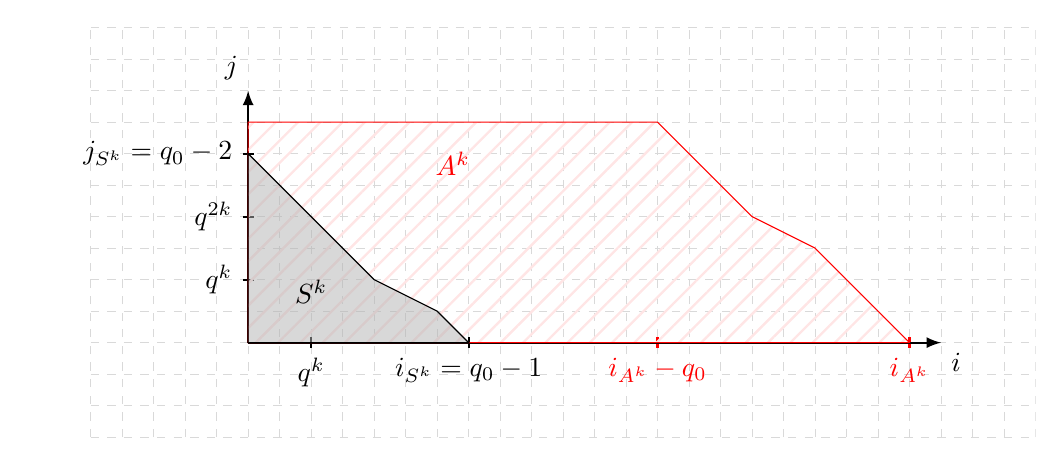
\begin{tikzpicture}[scale=0.4]
	\def\qO{8};
	\def\q{2};
	\def\iAk{21};
	\def\largeur{\iAk+4}
	\def\hauteur{\qO+2}
\clip (-7,-3) rectangle (\largeur,\hauteur); % Clips the picture...
\draw[style=help lines,dashed,opacity=0.3] (-5,-3) grid[step=1cm] (\largeur,\hauteur); % Draws a grid in the new coordinates.

%Sommets des polygones
\coordinate (A) at (\iAk,0) {};
\coordinate (B) at (\iAk-\qO,\qO-1) {};
\coordinate (C) at (0,\qO-1) {};
\coordinate (D) at (0,\qO-2) {};
\coordinate (E) at (\qO-1,0) {} ;
\coordinate (F) at (2*\q,\q) {};
\coordinate (G) at (\qO-2,1) {};
\coordinate (H) at (18,3) {};
\coordinate (I) at (16,4) {};


%Marqueurs sur l'axe vertical
\draw[thick] (5pt,\q) -- (-5pt,\q) node[anchor=east] {$q^k$} ;
\draw[thick] (5pt,\qO-4) -- (-5pt,\qO-4) node[anchor=east] {$q^{2k}$} ;
\draw[thick] (5pt,\qO-2) -- (-5pt,\qO-2) node[anchor=east] {$j_{S^k}=q_0-2$} ;


%Marqueurs sur l'axe horizontal
\draw[thick,red] (\iAk-\qO,5pt) -- (\iAk-\qO,-5pt) node[anchor=north] {$i_{A^k}-q_ 0$} ;
\draw[thick,red] (\iAk,5pt) -- (\iAk,-5pt) node[anchor=north] {$i_{A^k}$} ;
\draw[thick] (\q,5pt) -- (\q,-5pt) node[anchor=north] {$q^k$} ;
\draw[thick] (\qO-1,5pt) -- (\qO-1,-5pt) node[anchor=north] {$i_{S^k}=q_0-1$} ;



%Axes
\draw [thick,-latex] (0,0) -- (0,\qO) node [above left] {$j$};
\draw [thick,-latex] (0,0) -- (\iAk+1,0) node [below right] {$i$};

%Formes
\filldraw [ pattern color=red!10,
	pattern={Lines[
	distance=2mm,
	angle=45,
	line width=0.3mm]},
	draw=red] (0,0) -- (A) -- (H) -- (I) -- (B) -- (C) -- cycle;
	
\node[red,yshift=-1.5em] at ($(B)!0.5!(C)$) {$A^k$};


\filldraw [fill=black!30, fill opacity=0.5, draw=black] ([c]0,0) -- ([c]E) -- ([c]G) -- ([c]F) -- ([c]D)-- cycle;

	\node[yshift=0.7em] at ($(0,0)!0.5!(F)$) {$S^k$};

 
\end{tikzpicture} 
\caption{Case $2k < \frac{m}{2}$}
\end{center}
\end{figure}
\begin{figure}[h]
\begin{center}
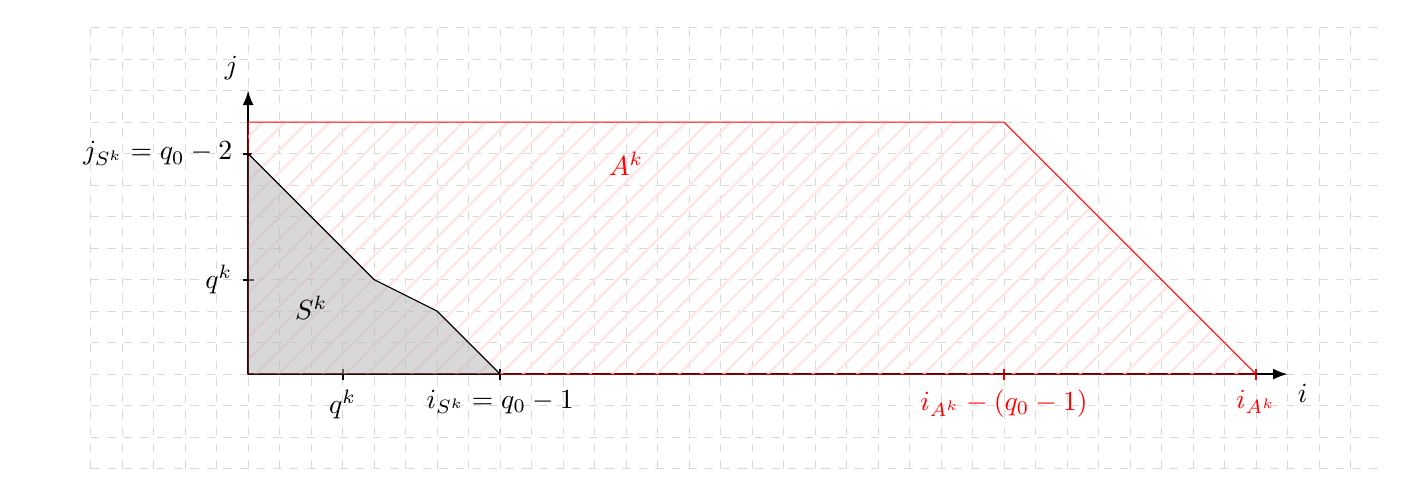
\begin{tikzpicture}[scale=0.4]
	\def\qO{9};
	\def\q{3};
	\def\iAk{32};
	\def\largeur{\iAk+4}
	\def\hauteur{\qO+2}
\clip (-7,-3) rectangle (\largeur,\hauteur); % Clips the picture...
\draw[style=help lines,dashed,opacity=0.3] (-5,-3) grid[step=1cm] (\largeur,\hauteur); % Draws a grid in the new coordinates.

%Sommets des polygones
%A^k
\coordinate (A) at (\iAk,0) {};
\coordinate (B) at (\iAk-\qO+1,\qO-1) {};
\coordinate (C) at (0,\qO-1) {};
%S^k
\coordinate (D) at (\qO-1,0) {};
\coordinate (E) at (\qO-3,2) {} ;
\coordinate (F) at (\q+1,\q) {};
\coordinate (G) at (0,\qO-2) {};



%Marqueurs sur l'axe vertical
\draw[thick] (5pt,\q) -- (-5pt,\q) node[anchor=east] {$q^k$} ;

\draw[thick] (5pt,\qO-2) -- (-5pt,\qO-2) node[anchor=east] {$j_{S^k}=q_0-2$} ;


%Marqueurs sur l'axe horizontal
\draw[thick,red] (\iAk-\qO+1,5pt) -- (\iAk-\qO+1,-5pt) node[anchor=north] {$i_{A^k}-(q_ 0-1)$} ;
\draw[thick,red] (\iAk,5pt) -- (\iAk,-5pt) node[anchor=north] {$i_{A^k}$} ;
\draw[thick] (\q,5pt) -- (\q,-5pt) node[anchor=north] {$q^k$} ;
\draw[thick] (\qO-1,5pt) -- (\qO-1,-5pt) node[anchor=north] {$i_{S^k}=q_0-1$} ;



%Axes
\draw [thick,-latex] (0,0) -- (0,\qO) node [above left] {$j$};
\draw [thick,-latex] (0,0) -- (\iAk+1,0) node [below right] {$i$};

%Formes
\filldraw [ pattern color=red!10,
pattern={Lines[
	distance=2mm,
	angle=45,
	line width=0.3mm]},
	draw=red] (0,0) -- (A) -- (B) -- (C) -- cycle;
	
\node[red,yshift=-1.5em] at ($(B)!0.5!(C)$) {$A^k$};
	
	

\filldraw [fill=black!30, fill opacity=0.5, draw=black] ([c]0,0) -- ([c]D) -- ([c]E) -- ([c]F) -- ([c]G)-- cycle;

	\node[yshift=0.7em] at ($(0,0)!0.5!(F)$) {$S^k$};
 
\end{tikzpicture} 
\caption{Case $2k \geq \frac{m}{2}$}
\end{center}
\end{figure}

At this stage of the proof, it remains to prove that every point in $A^k$ belongs to some $S^k_{(i_2,j_2)}$, for $(i_2,j_2) \in S^k$. Note that in the plan, the set $S^k_{(i_2,j_2)}$ has the same shape as $S^k$, but its bottom left point has coordinates $(i_2,j_2)$ instead of the origin $(0,0)$. We will prove first it the case $2k \geq \frac{m}{2}$, similar arguments works for the other one. Taking a point $b(i_b,j_b)$ in $A^k$, we can distinguish two cases:

\begin{itemize}
    \item[$\star$] If $i_b < (q_0-1)q^k$, then $b$ is in the rectangle delimited by $(0,0), ((q_0-1)q^k-1,0), ((q_0-1)q^k,q_0-1)$ and $(0,q_0-1)$ (note that $(q_0-1)q^k=i_{A^k}-(q_0-1)$). Let us write
    \[i_b = \alpha q^k+\gamma, \quad \mathrm{with} \quad \gamma < q^k.\]
    We want to show that all points $(i_b,0),\cdots,(i_b,q_0-1) \in B^k$, to ensure that $b$ is also. In particular, if we denote by $j^*:=\max \{j \ | \ (\alpha,j) \in S^k\} = \left\lfloor \frac{s-\alpha q_0}{q_0+1}\right\rfloor$, we will show that all theses points are in 
    \[\bigcup_{j=0}^{j^*} S^k_{(\alpha,j)}.\]
    In fact, let $0 \leq j \leq j^*$. Then the set $ S^k_{(\alpha,j)}$ contains $(i_b,jq^k+r)$ for any $0 \leq r \leq q_0-2-\gamma$ (note that we have no problem with the gap appearing in $S^k$ since it occurs at $q^k$, in which case we rather consider the set  $ S^k_{(\alpha+1,j)}$ instead of  $ S^k_{(\alpha,j)}$) . Since $(j+1)q^k \leq jq^k + (q_0-2-\gamma)+1$ (the equality is attained with $q^k=q=2$ and $q_0=4$), we do not miss any integer from $S^k_{(\alpha,j)}$ to $S^k_{(\alpha,j+1)}$; it remains to show that $j^*$ is big enough to reach the maximal ordinate this way, which is $q_0-1$. Again, the worst case (minimal value of $j^*$) is attained when $\alpha = q_0-2$ is maximal. In this situation, we have 
    \[j^* = \left\lfloor \dfrac{q_0+q^k-1}{q_0+1}\right\rfloor \geq 1,\]
    and the biggest ordinate reached is $q^k+q_0-2-\gamma \geq q_0-1$, since $\gamma < q^k$. To sum up, we are able to reach all points in the rectangle. In the picture below, we can see that $A \in S^k_{(q_0-4,1)}$. 

/%\jade{Pas sûre qu'appeler le point $A$ soit une bonne idée...}

\begin{figure}[h]
\begin{center}
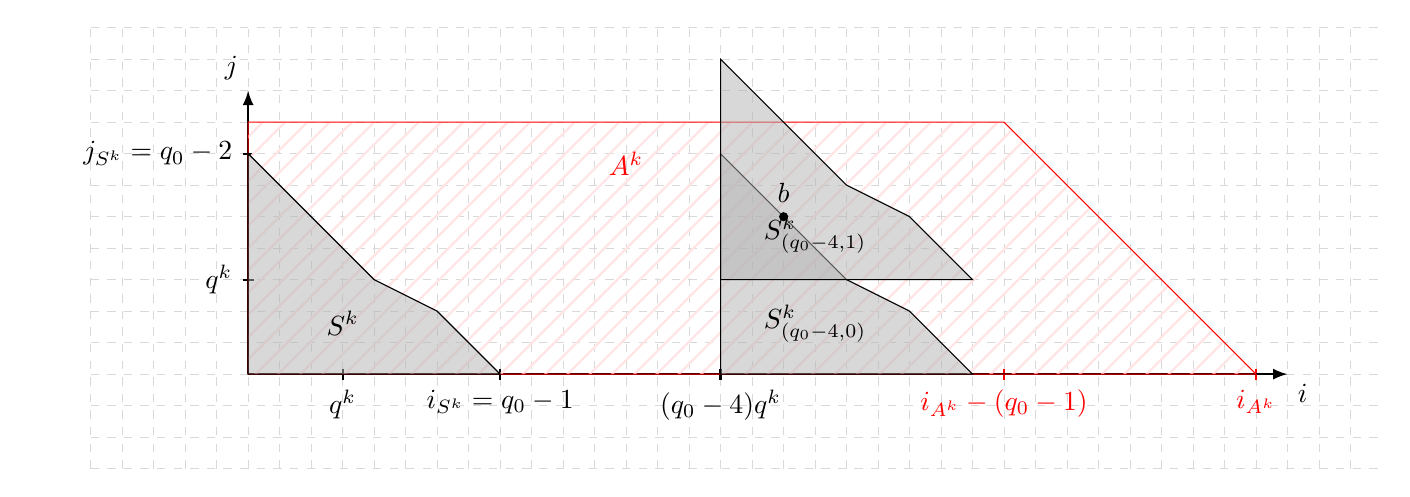
\begin{tikzpicture}[scale=0.4]
	\def\qO{9};
	\def\q{3};
	\def\iAk{32};
	\def\largeur{\iAk+4}
	\def\hauteur{\qO+2}
\clip (-7,-3) rectangle (\largeur,\hauteur); % Clips the picture...
\draw[style=help lines,dashed,opacity=0.3] (-5,-3) grid[step=1cm] (\largeur,\hauteur); % Draws a grid in the new coordinates.

%Sommets des polygones
%A^k
\coordinate (A) at (\iAk,0) {};
\coordinate (B) at (\iAk-\qO+1,\qO-1) {};
\coordinate (C) at (0,\qO-1) {};
%S^k
\coordinate (D) at (\qO-1,0) {};
\coordinate (E) at (\qO-3,2) {} ;
\coordinate (F) at (\q+1,\q) {};
\coordinate (G) at (0,\qO-2) {};


%finir le rectangle
\coordinate (H) at (\iAk-\qO,0) {};


%Marqueurs sur l'axe vertical
\draw[thick] (5pt,\q) -- (-5pt,\q) node[anchor=east] {$q^k$} ;
%\draw[thick] (5pt,\qO-4) -- (-5pt,\qO-4) node[anchor=east] {$q^{2k}$} ;
\draw[thick] (5pt,\qO-2) -- (-5pt,\qO-2) node[anchor=east] {$j_{S^k}=q_0-2$} ;


%Marqueurs sur l'axe horizontal
\draw[thick,red] (\iAk-\qO+1,5pt) -- (\iAk-\qO+1,-5pt) node[anchor=north] {$i_{A^k}-(q_ 0-1)$} ;
\draw[thick,red] (\iAk,5pt) -- (\iAk,-5pt) node[anchor=north] {$i_{A^k}$} ;
\draw[thick] (\q,5pt) -- (\q,-5pt) node[anchor=north] {$q^k$} ;
\draw[thick] (\qO-1,5pt) -- (\qO-1,-5pt) node[anchor=north] {$i_{S^k}=q_0-1$} ;
\draw[thick] (5*\q,5pt) -- (5*\q,-5pt) node[anchor=north] {$(q_0-4)q^k$} ;


%Axes
\draw [thick,-latex] (0,0) -- (0,\qO) node [above left] {$j$};
\draw [thick,-latex] (0,0) -- (\iAk+1,0) node [below right] {$i$};

%Formes
\filldraw [ pattern color=red!10,
pattern={Lines[
	distance=2mm,
	angle=45,
	line width=0.3mm]},
	draw=red] (0,0) -- (A) -- (B) -- (C) -- cycle;
	
% \filldraw [ pattern color=red!10,
% pattern={Lines[
% 	distance=2mm,
% 	angle=45,
% 	line width=0.3mm]},
% 	draw=blue] (23,0) -- (23,8) -- cycle;	
	
	\node[red,yshift=-1.5em] at ($(B)!0.5!(C)$) {$A^k$};

% \filldraw [ pattern color=black!20,
% pattern={Lines[
% 	distance=3mm,
% 	angle=45,
% 	line width=0.3mm]},
% draw=black] (0,0) -- (D) -- (E) -- (F) -- (G)-- cycle;

\foreach \coord in{(0,0),({\q*(\qO-4)},0),({\q*(\qO-4)},\q)} {
\begin{scope}[every coordinate/.style={shift={\coord}}]
	\filldraw [fill=black!30, fill opacity=0.5, draw=black] ([c]0,0) -- ([c]D) -- ([c]E) -- ([c]F) -- ([c]G)-- cycle;
\end{scope}
}

	\node[yshift=0.7em] at ($(0,0)!0.5!(E)$) {$S^k$};
	\node[yshift=0.7em] at ($(0,0)!0.5!(E)+({\q*(\qO-4)},0)$) {$S^k_{(q_0-4,0)}$};
	\node[yshift=0.5em] at ($(0,0)!0.5!(E)+({\q*(\qO-4)},\q)$) {$S^k_{(q_0-4,1)}$};

% un point A
\node[draw,circle,inner sep=1pt,fill,black,label=$b$] at (17,5) {};


\end{tikzpicture} 
\end{center}
\caption{Example with $2k \geq \frac{m}{2}$ and $i_b \leq (q_0-1)q^k$}
\end{figure}

 \item[$\star$] Else, we have $q^k(q_0-1) \leq i_b \leq (q^k+1)(q_0-1)$, i.e $b$ is in the triangle delimited by the points $((q_0-1)q^k,0)$, $((q_0-1)(q^k+1),0)$ and $((q_0-1)q^k,q_0-1)$, which we denote $\Delta$ from now on. We claim the following:
 \[ \forall \delta \in \{1,..,q^k\} \ , \ S^k_{(q_0-\delta,\delta-1)} \in B^k.\]
 To prove this, it suffices to show that $(q_0-\delta,\delta-1) \in S^k$, which is true since
 \[q_0(q_0-\delta) + \delta(q_0+1) = q_0(q_0-1)+\delta-1 \leq s.\]
 Next, we aim to prove
 \begin{equation} \label{counting}
 \Delta \subseteq \bigcup_{\delta=1}^{q^k} S^k_{(q_0-\delta,\delta-1)}.
 \end{equation}
 To do that, we start by counting the points in $\Delta$ and $S^k_{(q_0-1,0)}$. A short computation gives
 \[ \# \Delta = \dfrac{q_0(q_0+1)}{2} \quad \mathrm{and} \quad \# S^k_{((q_0-1)q^k,0)} := \dim \calL(sP_{\infty}) = s+1-g(\calH) = \dfrac{q_0(q_0-1)}{2} + q^k.\]
By definition, $S^k_{(q_0-1,0)} \subseteq \Delta$, and since $\# (\Delta \backslash  S^k_{((q_0-1)q^k,0)}) = q_0-q^k$, there is only a few points left to care about.
 They are included in the line joining $((q_0-1)(q^k+1),0)$ and $((q_0-1)q^k,q_0-1)$ since all points of cordinates $(i_{A^k}-\mu,\mu) (0 \leq \mu \leq q_0-1)$ can not be in $S^k_{((q_0-1),0)})$. For these $q_0$ points, we write 
 \[ \mu = \mu_1q^k + \mu_2,\]
 with $\mu_2 < q^k$ and $\mu_1 \leq \left\lfloor\frac{q_0-1}{q^k}\right\rfloor \leq q^{m/2-k}-1 \leq q^k-1$ (recall $k \geq m/4$). Next, we claim:
 \[(i_{A^k}-\mu,\mu) \in S^k_{q_0-1-\mu_1,\mu} \subseteq \bigcup_{\delta=1}^{q^k} S^k_{(q_0-\delta,\delta-1)}.\]
 Remark that $i_{A^k}-\mu = (q_0-1-\mu_1)q^k+(q_0-1-\mu_2)$, so we are led to prove $((q_0-1-\mu_2),\mu_2) \in S^k$, which again olds since $\mu_2 < q^k$. Note that $q^k$ of these points are in $S^k_{((q_0-1),0)})$ (case $\mu_1=0)$, meaning that the remaining $q_0-q^k$ are in $(\Delta \backslash  S^k_{((q_0-1),0)})$, which proves \eqref{counting} (see the figure below to compare $\Delta$ and $\bigcup_{\delta=1}^{q^k} S^k_{(q_0-\delta,\delta-1)}$ on a example).
 
 \begin{figure}[h]
\begin{center}
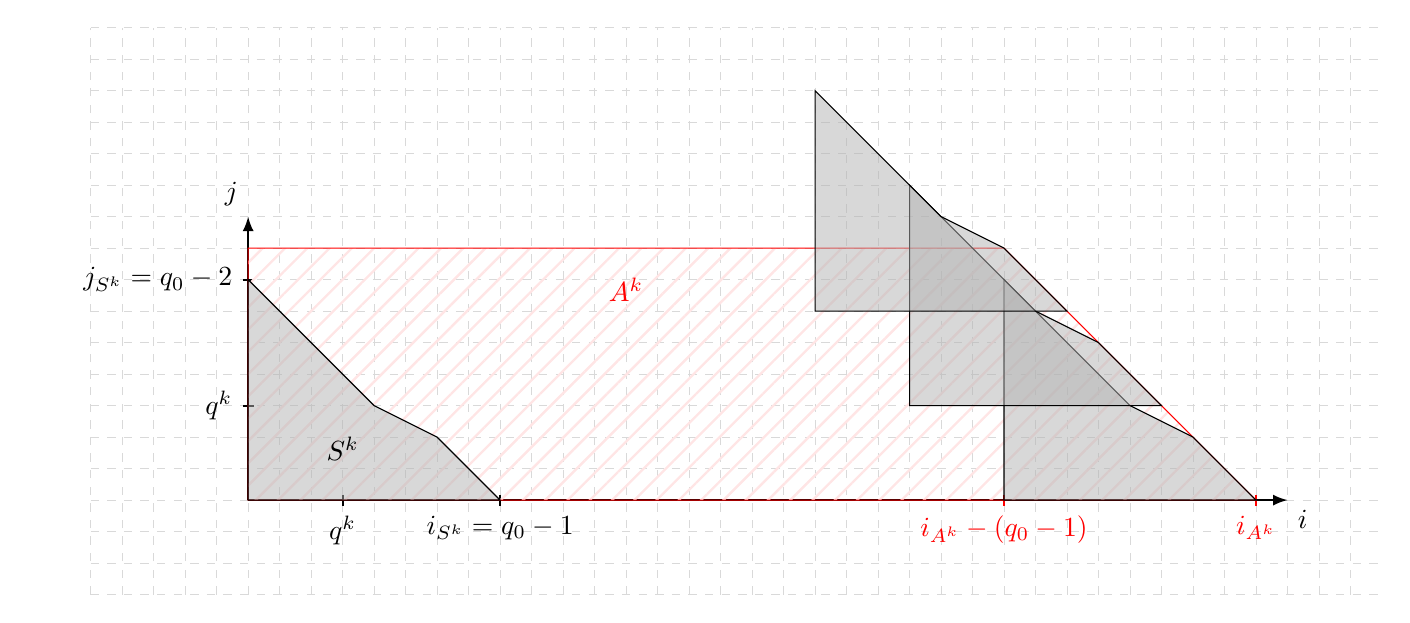
\begin{tikzpicture}[scale=0.4]
	\def\qO{9};
	\def\q{3};
	\def\iAk{32};
	\def\largeur{\iAk+4}
	\def\hauteur{\qO+6}
\clip (-7,-3) rectangle (\largeur,\hauteur); % Clips the picture...
\draw[style=help lines,dashed,opacity=0.3] (-5,-3) grid[step=1cm] (\largeur,\hauteur); % Draws a grid in the new coordinates.

%Sommets des polygones
%A^k
\coordinate (A) at (\iAk,0) {};
\coordinate (B) at (\iAk-\qO+1,\qO-1) {};
\coordinate (C) at (0,\qO-1) {};
%S^k
\coordinate (D) at (\qO-1,0) {};
\coordinate (E) at (\qO-3,2) {} ;
\coordinate (F) at (\q+1,\q) {};
\coordinate (G) at (0,\qO-2) {};


%finir le rectangle
\coordinate (H) at (\iAk-\qO,0) {};


%Marqueurs sur l'axe vertical
\draw[thick] (5pt,\q) -- (-5pt,\q) node[anchor=east] {$q^k$} ;
%\draw[thick] (5pt,\qO-4) -- (-5pt,\qO-4) node[anchor=east] {$q^{2k}$} ;
\draw[thick] (5pt,\qO-2) -- (-5pt,\qO-2) node[anchor=east] {$j_{S^k}=q_0-2$} ;


%Marqueurs sur l'axe horizontal
\draw[thick,red] (\iAk-\qO+1,5pt) -- (\iAk-\qO+1,-5pt) node[anchor=north] {$i_{A^k}-(q_ 0-1)$} ;
\draw[thick,red] (\iAk,5pt) -- (\iAk,-5pt) node[anchor=north] {$i_{A^k}$} ;
\draw[thick] (\q,5pt) -- (\q,-5pt) node[anchor=north] {$q^k$} ;
\draw[thick] (\qO-1,5pt) -- (\qO-1,-5pt) node[anchor=north] {$i_{S^k}=q_0-1$} ;



%Axes
\draw [thick,-latex] (0,0) -- (0,\qO) node [above left] {$j$};
\draw [thick,-latex] (0,0) -- (\iAk+1,0) node [below right] {$i$};

%Formes
\filldraw [ pattern color=red!10,
pattern={Lines[
	distance=2mm,
	angle=45,
	line width=0.3mm]},
	draw=red]  (0,0) -- (A) -- (B) -- (C) -- cycle;
	
\node[red,yshift=-1.5em] at ($(B)!0.5!(C)$) {$A^k$};	

\foreach \coord in{(0,0),(\iAk-\qO+1,0),(\iAk-\qO+1-\q,\q),(\iAk-\qO+1-2*\q,2*\q)} {
	\begin{scope}[every coordinate/.style={shift={\coord}}]
		\filldraw [fill=black!30, fill opacity=0.5, draw=black] ([c]0,0) -- ([c]D) -- ([c]E) -- ([c]F) -- ([c]G)-- cycle;
	\end{scope}
}

	\node[yshift=0.7em] at ($(0,0)!0.5!(E)$) {$S^k$};


 
\end{tikzpicture} 
\end{center}
\caption{Example with $2k \geq \frac{m}{2}$ and $i_b \geq (q_0-1)q^k$}

\end{figure}
\end{itemize}

We still have to deal with the case $2k < \frac{m}{2}$. Suppose it, then take a point $p(i_p,j_p) \in A^k$. Actually, we can proceed the exact same way if $i_p < q^k(q_0-1)$. It implies that we are left with $q^k(q_0-1) \leq i_p \leq (q^k+1)(q_0-1)$, i.e $p$ is in the polygone $\Gamma$ delimited by the points $(q^k(q_0-1),0)$, ($i_{A^k}$,0), ($i_{A^k}-(q^{2k}-1),q^{2k}-1)$, ($i_{A^k}-(q^{2k}+1,q^{2k})$ and $(q^k(q_0-1),q_0-2)$. As above, we have:
 \[ \forall \delta \in \{1,..,q^k\} \ , \ S^k_{(q_0-\delta,\delta-1)} \in B^k.\]
 and 
 \[S^k_{(q_0-1,0)} \subseteq \Delta.\]
This time, the same comutation trick gives
\[ \# \Gamma = \dfrac{q_0(q_0-1)}{2}+q^{2k} \quad \mathrm{and} \quad \# S^k_{(q_0-1,0)} = \dfrac{q_0(q_0-1)}{2}+q^{k}.\]
It implies $\# (\Gamma \backslash  S^k_{(q_0-1,0)}) = q^{2k}-q^k$. Again, those points are in the path joining ($i_{A^k}$,0) and  $(q^k(q_0-1),q_0-2)$, which contains $q_0-2$ points in total. Amoung them, some are already in $S^k_{(q_0-1,0)}$, exepted for (this is due to the gap at $q^{2k}$) 
\[ (i_{A^k}-\mu,\mu) \ , \ \mathrm{where} \ \mu \in \{q^k,\cdots,q^{2k}-1\}.\]
For such points, we write
\[\mu = \mu q^k + \mu_2 \ , \ \mathrm{with} \ \mu_1,\mu_2 < q^k,\]
and we claim that $(i_{A^k}-\mu,\mu) \in S^k_{((q_0-1)-\mu_1,\mu_1)} \in B^k$, which holds since both $\mu_1$ and $\mu_2$ are smaller than $q^k$. The picture bellow describes this case, and conclude the proof.

\begin{figure}[h]
\begin{center}
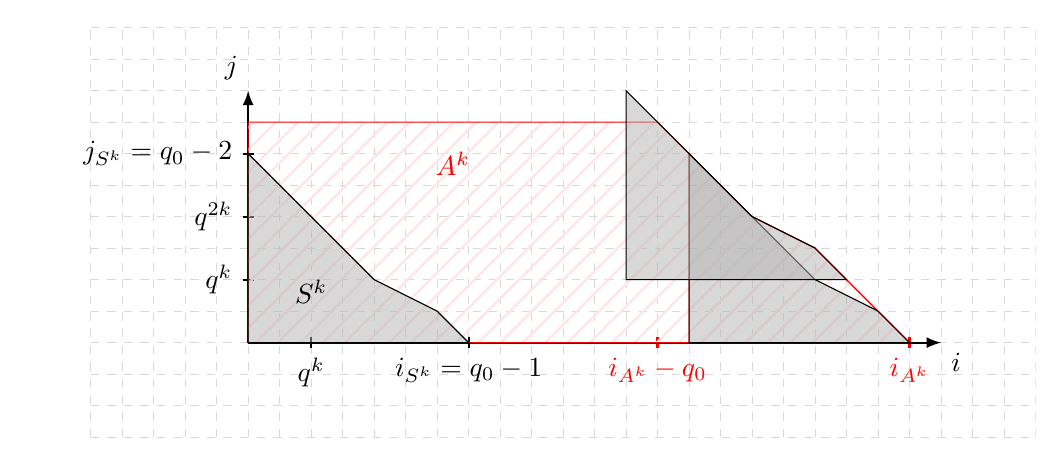
\begin{tikzpicture}[scale=0.4]
	\def\qO{8};
	\def\q{2};
	\def\iAk{21};
	\def\largeur{\iAk+4}
	\def\hauteur{\qO+2}
\clip (-7,-3) rectangle (\largeur,\hauteur); % Clips the picture...
\draw[style=help lines,dashed,opacity=0.3] (-5,-3) grid[step=1cm] (\largeur,\hauteur); % Draws a grid in the new coordinates.

%Sommets des polygones
\coordinate (A) at (\iAk,0) {};
\coordinate (B) at (\iAk-\qO,\qO-1) {};
\coordinate (C) at (0,\qO-1) {};
\coordinate (D) at (0,\qO-2) {};
\coordinate (E) at (\qO-1,0) {} ;
\coordinate (F) at (2*\q,\q) {};
\coordinate (G) at (\qO-2,1) {};
\coordinate (H) at (18,3) {};
\coordinate (I) at (16,4) {};


%Marqueurs sur l'axe vertical
\draw[thick] (5pt,\q) -- (-5pt,\q) node[anchor=east] {$q^k$} ;
\draw[thick] (5pt,\qO-4) -- (-5pt,\qO-4) node[anchor=east] {$q^{2k}$} ;
\draw[thick] (5pt,\qO-2) -- (-5pt,\qO-2) node[anchor=east] {$j_{S^k}=q_0-2$} ;


%Marqueurs sur l'axe horizontal
\draw[thick,red] (\iAk-\qO,5pt) -- (\iAk-\qO,-5pt) node[anchor=north] {$i_{A^k}-q_ 0$} ;
\draw[thick,red] (\iAk,5pt) -- (\iAk,-5pt) node[anchor=north] {$i_{A^k}$} ;
\draw[thick] (\q,5pt) -- (\q,-5pt) node[anchor=north] {$q^k$} ;
\draw[thick] (\qO-1,5pt) -- (\qO-1,-5pt) node[anchor=north] {$i_{S^k}=q_0-1$} ;



%Axes
\draw [thick,-latex] (0,0) -- (0,\qO) node [above left] {$j$};
\draw [thick,-latex] (0,0) -- (\iAk+1,0) node [below right] {$i$};

%Formes
\filldraw [ pattern color=red!10,
	pattern={Lines[
	distance=2mm,
	angle=45,
	line width=0.3mm]},
	draw=red] (0,0) -- (A) -- (H) -- (I) -- (B) -- (C) -- cycle;
	
\filldraw [ pattern color=red!10,
	pattern={Lines[
	distance=2mm,
	angle=45,
	line width=0.3mm]},
	draw=red] (14,0) -- (21,0) -- (18,3) -- (16,4) -- (14,6)  -- cycle;
	
\filldraw[fill=black!30, fill opacity=0.5, draw=black] (14,0) -- (21,0) -- (20,1) -- (18,2) -- (14,6)  -- cycle;

\filldraw[fill=black!30, fill opacity=0.5, draw=black] (12,2) -- (19,2) -- (18,3) -- (16,4) -- (12,8)  -- cycle;
	
\node[red,yshift=-1.5em] at ($(B)!0.5!(C)$) {$A^k$};


\filldraw [fill=black!30, fill opacity=0.5, draw=black] ([c]0,0) -- ([c]E) -- ([c]G) -- ([c]F) -- ([c]D)-- cycle;

	\node[yshift=0.7em] at ($(0,0)!0.5!(F)$) {$S^k$};

 
\end{tikzpicture} 
\caption{Example with $2k < \frac{m}{2}$ and $i_b \geq q^k(q_0-1)$}
\end{center}
\end{figure}

\end{proof}

\newpage















\begin{rq1} 
	In the picture below, you can find a counter-example in the case $B^k \ne A^k$ if $s$ does not reach the bound given in Proposition \ref{prop_avec_dessins}. \jade{Here, with $s=\mu_g+q^k-1$, we can see that some monomials $x^iy^j \in \calL((q+1)sP_\infty)$ cannot be written as a product $x^{i_1+qi_2}y^{j_1+qj_2}$ for $(i_r,j_r) \in S_k$.}
	\begin{figure}[h]
		\begin{center}
			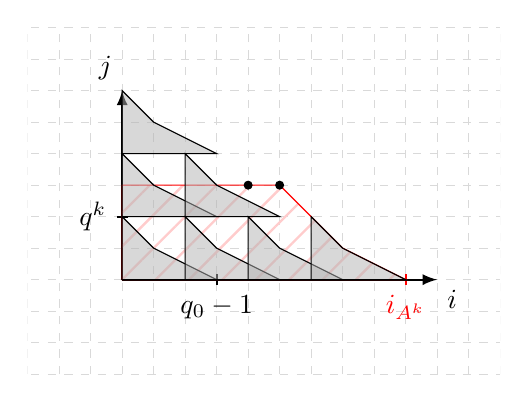
\begin{tikzpicture}[scale=0.4]
				\def\qO{4};
				\def\q{2};
				\def\iAk{9};
				\def\largeur{\iAk+3}
				\def\hauteur{\qO+4}
				\clip (-3,-3) rectangle (\largeur,\hauteur); % Clips the picture...
				\draw[style=help lines,dashed,opacity=0.3] (-5,-3) grid[step=1cm] (\largeur,\hauteur); % Draws a grid in the new coordinates.
				
				%Sommets des polygones
				%A^k
				\coordinate (A) at (\iAk,0) {};
				\coordinate (B) at (\iAk-\qO,\qO-1) {};
				\coordinate (C) at (0,\qO-1) {};
				%S^k
				\coordinate (D) at (\qO-1,0) {};
				\coordinate (E) at (\qO-3,2) {} ;
				\coordinate (F) at (\q+1,\q) {};
				\coordinate (G) at (0,\qO-2) {};
				
				
				%finir le rectangle
				\coordinate (H) at (\iAk-\qO,0) {};
				
				
				%Marqueurs sur l'axe vertical
				\draw[thick] (5pt,\q) -- (-5pt,\q) node[anchor=east] {$q^k$} ;
				%\draw[thick] (5pt,\qO-4) -- (-5pt,\qO-4) node[anchor=east] {$q^{2k}$} ;
				
				
				
				%Marqueurs sur l'axe horizontal
				%\draw[thick,red] (\iAk-\qO+1,5pt) -- (\iAk-\qO+1,-5pt) node[anchor=north] {$i_{A^k}-(q_ 0-1)$} ;
				\draw[thick,red] (\iAk,5pt) -- (\iAk,-5pt) node[anchor=north] {$i_{A^k}$} ;
				% \draw[thick] (\q,5pt) -- (\q,-5pt) node[anchor=north] {$q^k$} ;
				\draw[thick] (\qO-1,5pt) -- (\qO-1,-5pt) node[anchor=north] {$q_0-1$} ;
				
				
				
				%Axes
				\draw [thick,-latex] (0,0) -- (0,\qO+2) node [above left] {$j$};
				\draw [thick,-latex] (0,0) -- (\iAk+1,0) node [below right] {$i$};
				
				%Formes
				\filldraw [ pattern color=red!20,
				pattern={Lines[
					distance=3mm,
					angle=45,
					line width=0.3mm]},
				draw=red] (0,0) -- (9,0) -- (7,1) -- (5,3) -- (0,3)-- cycle;
				
				\foreach \i in {0,1,2,3}{
					\filldraw [fill=black!30, fill opacity=0.5, draw=black] (2*\i,0) -- (3+2*\i,0) -- (1+2*\i,1) -- (2*\i,2)-- cycle;
				}
				
				\foreach \i in {0,1}{
					\filldraw [fill=black!30, fill opacity=0.5, draw=black] (2*\i,2) -- (3+2*\i,2) -- (1+2*\i,3) -- (2*\i,4)-- cycle;
				}
				
				\filldraw [fill=black!30, fill opacity=0.5, draw=black] (0,4) -- (3,4) -- (1,5) -- (0,6)-- cycle;
				
				\node[draw,circle,inner sep=1pt,fill,black] at (4,3) {};
				\node[draw,circle,inner sep=1pt,fill,black] at (5,3) {};
				
				
				
			\end{tikzpicture} 
		\end{center}
		\caption{Counter-example with $(q,q_0,s,k)= (2,4,1,\mu_g+q-1)$}
		
	\end{figure}
\end{rq1}

\newpage


































\begin{rq1}
The difference between Propositions \ref{result_with_valuations} and \ref{powers_of_q's_case} is that in the second case, we are only able to give a sufficient condition.
\end{rq1} 

From this two results, we deduce:

\begin{coro1} \label{coro2}
Let $\calC = C_{\calL}(\calH,\calP,sP_{\infty})$ be an AG-code on $\calH$ over $\mathbb{F}_{q^m}=\mathbb{F}_{q_0^2}$, assciated to a support $\calP$ of length $n$ and to the one-point divisor $sP_{\infty}$. Denote by $g:=g(\calH)=\frac{q_0(q_0-1)}{2}$ and $\mu_g := q_0(q_0-1)-1$ the biggest gap number of $P_{\infty}$. 
\begin{itemize}
    \item[(i)] If $s \geq \mu_g + q_0^2$, then we have 
        \[\Tr(\calC \star \calC) \subseteq \Tr(\calC \star \calC^q) \subseteq \cdots \subseteq \Tr(\calC \star \calC^{q_0}),\]
        and thus 
        \[\Tr(\calC)^{\star 2} \subseteq \Tr(\calC \star \calC^{q_0}).\]
    \item[(ii)] If $\mu_g < s < \mu_g +q_0^2$, denote by $f:= \max\{k \in \{0,\cdots,\frac{m}{2}-1\} : s \geq \mu_g + q^k\}$. In this case, we have 
        \[\Tr(\calC \star \calC) \subseteq \Tr(\calC \star \calC^q) \subseteq \cdots \subseteq \Tr(\calC \star \calC^{q^f}),\]
          and then
        \[\Tr(\calC)^{\star 2} \subseteq \Tr(\calC \star \calC^{q^f}) + \sum\limits_{i=f+1}^{m/2} \Tr(\calC \star \calC^{q^i}).\]
\end{itemize}
\end{coro1}

\begin{proof}
$(i)$ is a consequence of Proposition \ref{result_with_valuations} in the case $i=1$ (note that the result also holds without the Trace operator), while $(ii)$ uses Proposition \ref{powers_of_q's_case} several times. In both cases, we conclude get a result on $\Tr(\calC)^{\star 2}$ by using Theorem \ref{th1}.
\end{proof}

Using the above Corollary and Lemma \ref{known_bounds}, we can prove the following theorem, that gives an upper bound on the dimension of the trace of the square of the dual of our one-point Hermitian SSAG-code which can be compared to the one given in Corollary \ref{square_ssag_bound}.

\begin{thm} \label{sup_bounds_on_codes}
We keep notations as in Corollary 2, and denote by $k$ the dimension of $\calC$ over $\fqm$.
\begin{itemize}
\item[(i)] If $s \geq \mu_g + q_0^2$, then 
\[ \dim_{\fq}(\Tr(\calC))^{\star 2} \leq \binom{mk+1}{2} - \dfrac{m}{2} (k(mk-1)-2q_0s).\]
\item[(ii)] If $\mu_g < s < \mu_g +q_0^2$, recall that $f:= \max\{k \in \{0,\cdots,\frac{m}{2}-1\} : s \geq \mu_g + q^k\}$. Then 
\[ \dim_{\fq}(\Tr(\calC))^{\star 2} \leq \binom{mk+1}{2} - \dfrac{m}{2}(k(2fk-1)-2q^fs).\]
\end{itemize}
\end{thm}

\begin{proof}
\begin{itemize}
    \item[$(i)$] From Corollary 2 $(i)$, we have $\Tr(\calC)^{\star 2} \subseteq \Tr(\calC \star \calC^{q_0}).$ Moreover, we proved in Proposition \ref{result_with_valuations} that under the hypothesis on $s$, we had
      \[ \calC \star \calC^{q_0} = \calC^{q_0+1} := C_{\calL}(\calH,\calP,(q_0+1)sP_{\infty}),\]
      which is a dimension $(q_0+1)s + 1 - g(\calH)$ code, as follows from the Riemann-Roch theorem. As a result, we can estimate
      \begin{align*}
           \dim_{\fq}(\Tr(\calC))^{\star 2} &\leq \dim_{\fq}(\Tr(\calC^{q_0+1})) \\
                                            & = m((q_0+1)s + 1 - g(\calH)) \\
                                            & = m (k+q_0 s) \\
                                            & = \binom{mk+1}{2} + \dfrac{m}{2}(2k+2q_0s-k(mk+1)) \\
                                            &= \binom{mk+1}{2} - \dfrac{m}{2} (k(mk-1)-2q_0s).
      \end{align*}
      \item[$(ii)$] Corollary 2 $(ii)$ together with Proposition \ref{powers_of_q's_case} gives 
       \[\Tr(\calC)^{\star 2} \subseteq \Tr(\calC \star \calC^{q^f}) + \sum\limits_{i=f+1}^{m/2} \Tr(\calC \star \calC^{q^i})\]
       and 
        \[ \calC \star \calC^{q^f} = \calC^{q^f+1} := C_{\calL}(\calH,\calP,(q^f+1)sP_{\infty}).\]
        Since the latter code has dimension $(q^f+1)s+1-g(\calH)=k+q^fs$, we have (using twice Lemma \ref{known_bounds})
         \begin{align*}
           \dim_{\fq}(\Tr(\calC))^{\star 2} &\leq \dim_{\fq}(\Tr(\calC^{q_f+1})) +  \sum\limits_{i=f+1}^{m/2} \dim_{\fq}(\Tr(\calC \star \calC^{q^i}))\\
                                            &\leq m \cdot (k + q^fs) + m  \sum\limits_{i=f+1}^{m/2} \dim_{\fqm}(\calC \star \calC^{q^i}) \\
                                            &\leq m \cdot \left(k+q^fs + k^2 \left(\frac{m}{2}-f\right)\right). \\
                                            &= \dfrac{m}{2}(2k+2q^fs+mk^2-2k^2f) \\
                                         &=\binom{mk+1}{2}-\dfrac{m}{2}(k(2fk-1)-2q^fs).
      \end{align*}
\end{itemize}
\end{proof}

Note that, as explained at the beggining of this Section, Theorem \ref{sup_bounds_on_codes} above gives upper bounds on dimension of the square of the dual of the \textrm{SSAG}-code
\[\mathrm{SSAG}_{q}(\calH,\calP,D^{\perp}),\]
where $D^{\perp} = s' P_{\infty}$ and $s'= q_0^3+q_0^2-q_0-2-s$.

% The following Corollary traduce them in terms of SSAG code and the integer $s'$.

% \begin{coro1}
% \end{coro1}

\clearpage
\bibliography{biblio}
\bibliographystyle{alpha}



\end{document}
